\section{Model A - CNN Created From Scratch}
\subsection{Architecture}
Our model architecture is shown in \autoref{fig:ModelAGraph}.
\begin{figure}[h!]
    \centering
    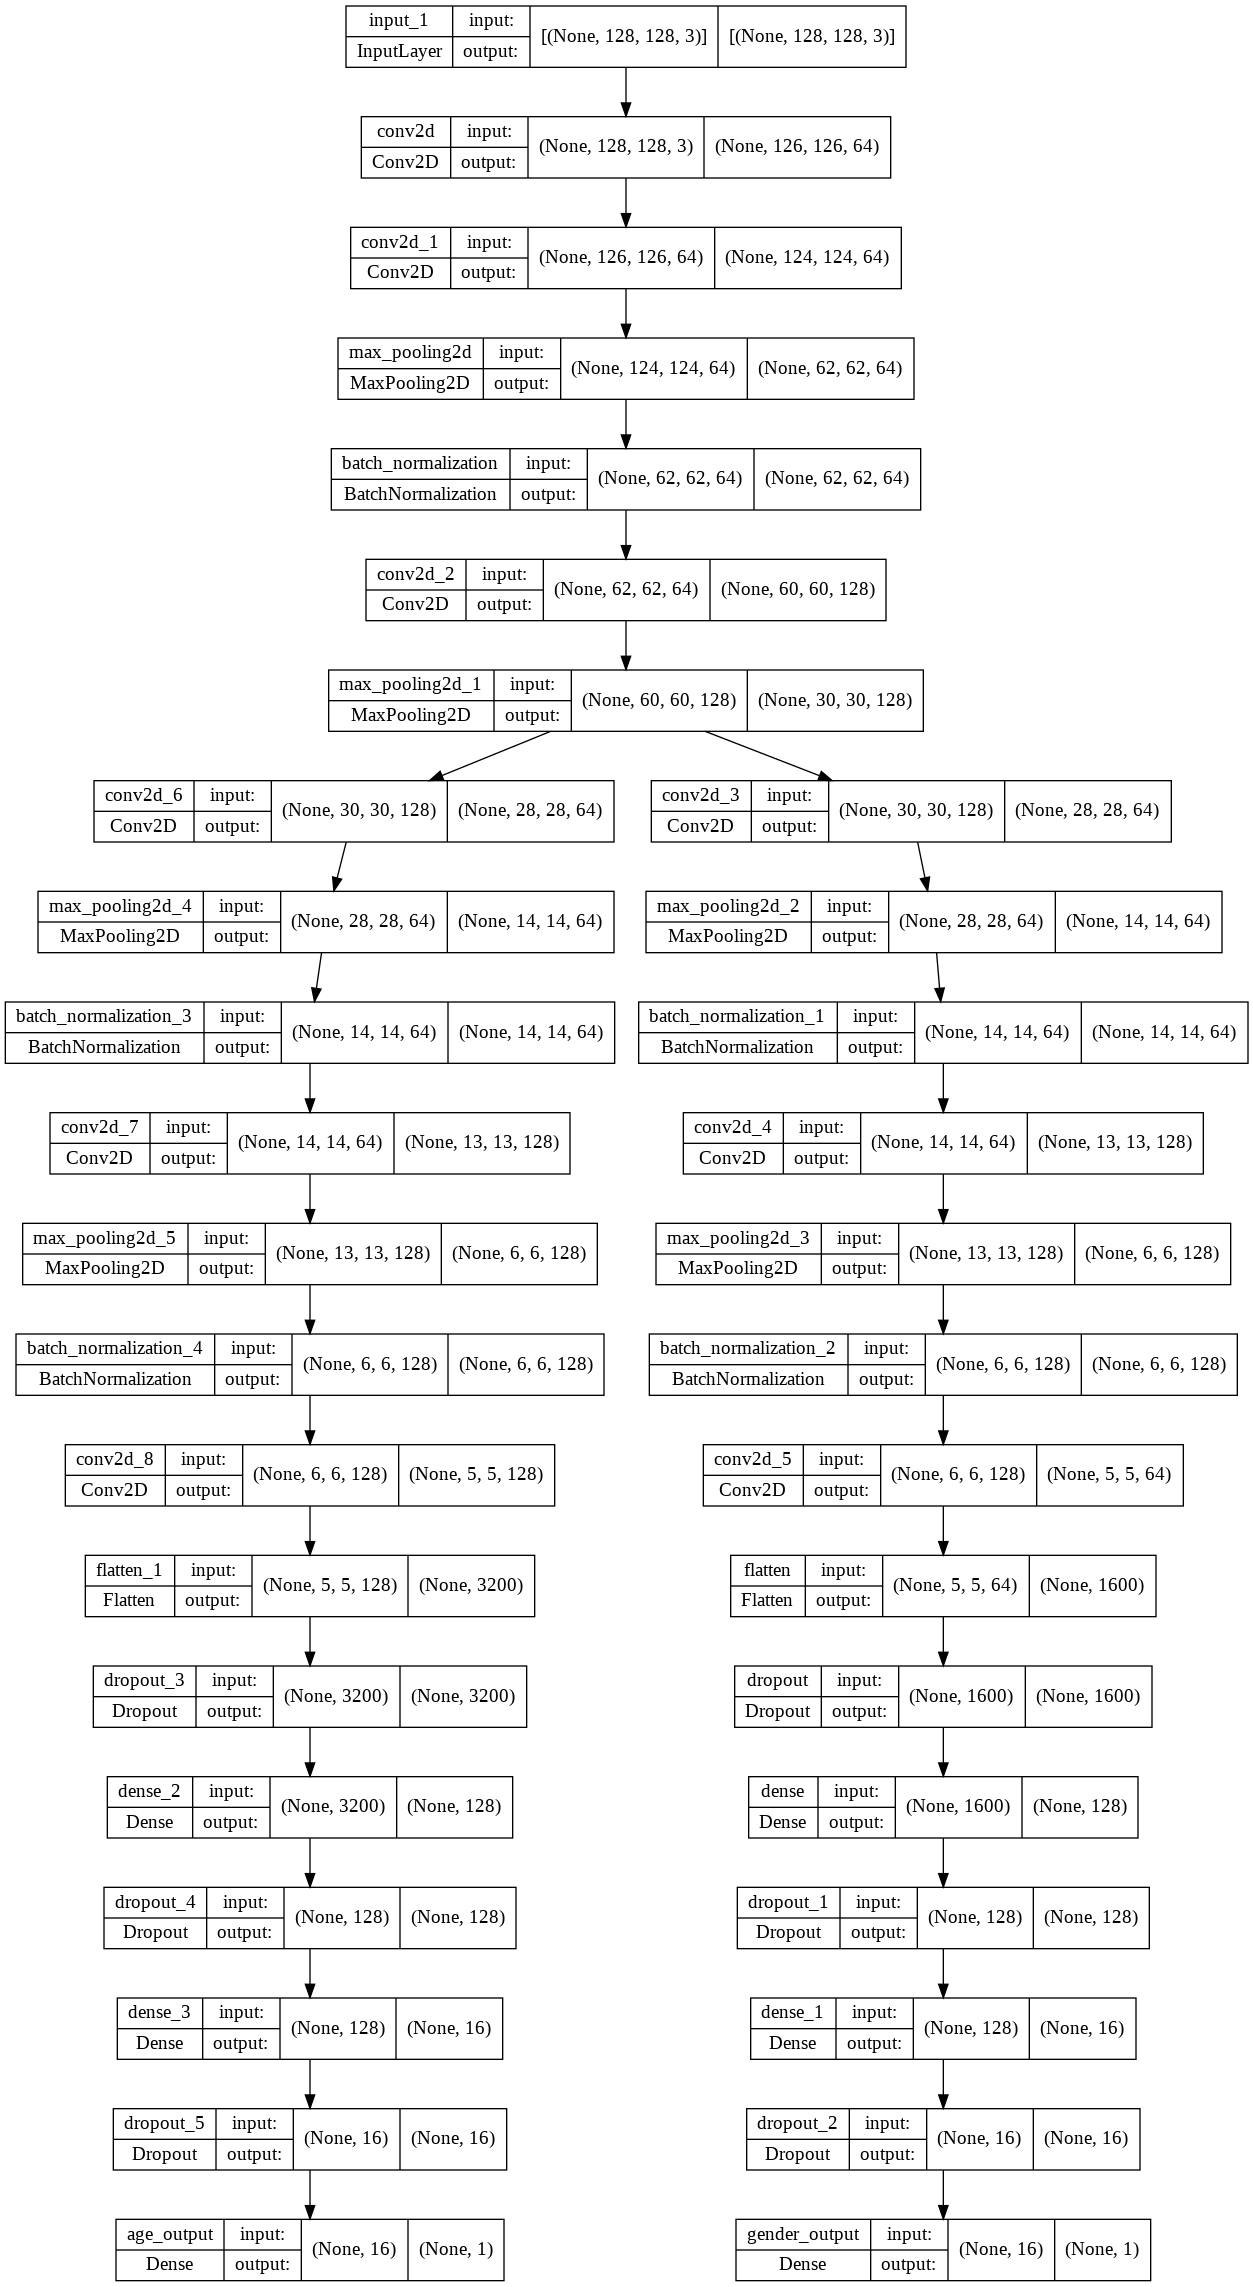
\includegraphics[height=0.95\textheight]{ModelA_Graph.png}
    \caption{The architecture for Model A.}
    \label{fig:ModelAGraph}
\end{figure}

It consists of a shared trunk of convolutional layers with relu activation. These layers are interspersed with maxpooling and batch normalisation layers.  
The output of this trunk is sent to different branches for age and gender prediction. 
The age and gender branches have the same architecture except for the number of filters in their final convolutional layers. 
Each branch has three convolutional layers interspersed with maxpooling and batch normalisation. 
The output of these convolutional layers is then flattened and fed into a 3 layer dense MLP. The final layer is a single node for the output. The output of the age branch has no activation and the output of the gender branch has a sigmoid activation. 


This architecture was chosen because the first layers of a CNN usually extract generic low-level features which are common to many images. 
Therefore using a shared trunk allows the network to use fewer parameters and helps reduce over-fitting.
The branches then allow the model to further extract higher level features specific to age or gender prediction. 
The convolutional layers extract features from the input, the maxpooling layers reduce the parameter count and the batchnorm layers help to prevent vanishing gradient issues. The dense layers are responsible for making sense of these extracted features in order to make predictions.

Measures employed to reduce over-fitting include the shared trunk as well as dropout and L2 regularisation on the dense layers.

\subsection{Training}
The model is trained to minimize a weighted average of losses from each branch. \\
The loss for the gender prediction output is binary cross entropy because it is a binary classification problem and the loss for the age prediction is mean squared error because it is a regression problem. 
Mean squared error was chosen over mean absolute error in order to penalise larger errors more than smaller ones. 
The average loss is weighted 1:100 towards gender prediction because typical gender losses seen during training were approximately 100 times smaller than the age losses.
This weighting was chosen so the model attempts to balance its training objectives without over-prioritising either age or gender. 
The model uses the Adam optimizer with a exponentially decaying learning rate to train for a total of 50 epochs. 

Hyper-parameters were tuned using the \verb|keras_tuner| library to minimise the validation loss. After tuning the tuned values were fixed and the model was rebuilt using them. The following hyper-parameters were tuned:
\begin{enumerate}
    \item Greyscale: Whether to apply a greyscale filter to the gender branch, both branches, or neither.
    \item Sigmoid Vs \verb|BinaryCrossEntropy| With logits: Whether to use a sigmoid activation on the gender branch or enable logits for the \verb|BinaryCrossEntropy| loss function.
    \item Initial Learning rate
    \item Feature depth of final convolution layer
    \item Dropout rate 
    \item Regularisation
\end{enumerate}
An output of the tuning can be found in the appendix here \autoref{appendix:Model_A_Hyper-Parameter_Tuning}

\subsection{Data}
The model is trained on data from the dataset provided. The data is augmented using the Keras \verb|ImageDataGenerator| to effectively increase the size of the dataset and prevent over-fitting. 
The augmentations used are rotation, zoom, and horizontal flipping. Pixel values were scaled between 0 and 1.

A 20\% validation split was used. The training and validation data were subject to the same preprocessing.

\subsection{Performance}
\autoref{fig:ModelAPerformanceAge} and \autoref{fig:ModelAPerformanceGender} show the training graphs. 
Our model shows good performance on both age and gender prediction. 
It achieves an accuracy of 93\% for gender prediction and a mean absolute error of 5.6 for age prediction on the training data.\\
However it can be seen that the model over-fits slightly and achieves slightly lower performance on the validation data, with an accuracy or 88\% for gender prediction and mean absolute error of 6.8 for age prediction. 
The gender branch can be seen to over-fit to a greater extent than the age branch.

The trace of the final training epoch is below.
\begin{verbatim}
Epoch 50/50
125/125 [==============================] 
- 41s 325ms/step 
- loss: 82.5588 
- age_output_loss: 55.1034 
- gender_output_loss: 0.1627 
- age_output_mean_absolute_error: 5.5780 
- gender_output_binary_accuracy: 0.9330 
- val_loss: 131.3783 
- val_age_output_loss: 90.0434 
- val_gender_output_loss: 0.3111 
- val_age_output_mean_absolute_error: 6.8350 
- val_gender_output_binary_accuracy: 0.8821
\end{verbatim}

\begin{figure}[h]
    \begin{subfigure}{\textwidth}
        \centering
        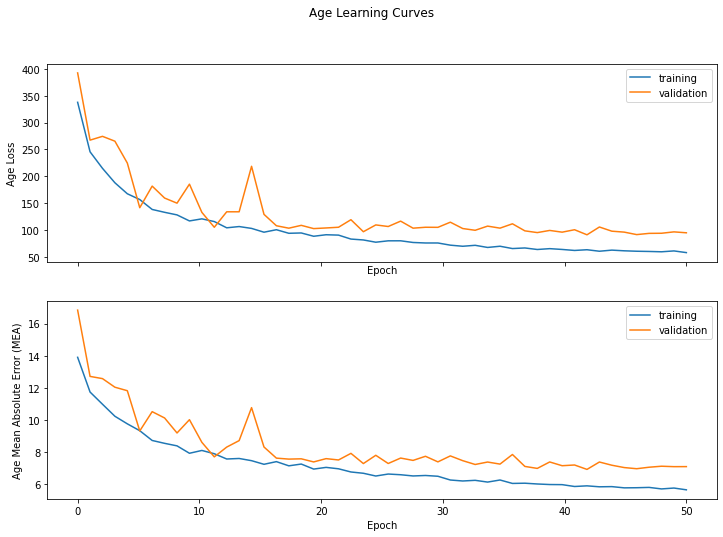
\includegraphics[height=0.45\textheight]{ModelA_AgeLearning_TunedHyperParams.png}
        \caption{\label{fig:ModelAPerformanceAge} The performance on age prediction for our model.}
    \end{subfigure}
    \begin{subfigure}{\textwidth}
        \centering
        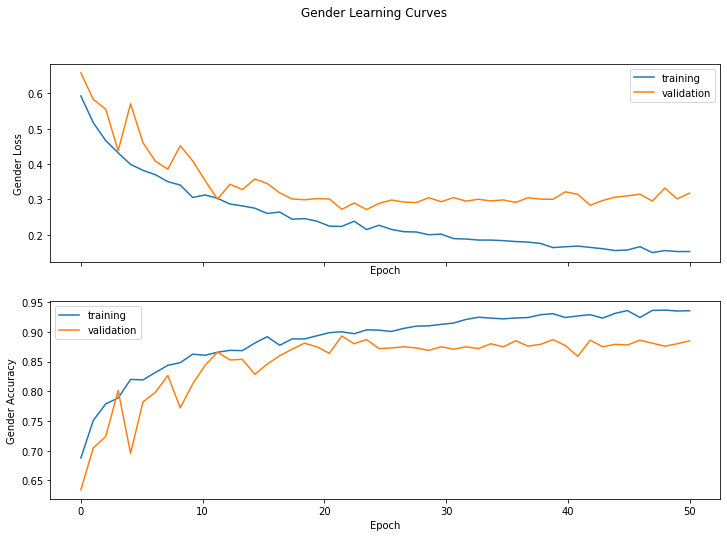
\includegraphics[height=0.45\textheight]{ModelA_GenderLearning_TunedHyperParams.png}
        \caption{\label{fig:ModelAPerformanceGender} The performance on gender prediction for our model.}
    \end{subfigure}
    \label{fig:ModelAPerformance}
    \caption{Learning curves observed training Model A}
\end{figure}
